

\chapter{Literature Survey}


\section{Geometric Approaches to Visual Odometry}

Since the invention of the pinhole camera, most cameras have captured 2D representations of a 3D world, meaning information about physical structure is lost. With the addition of a second viewpoint however we can learn a little more about the shape of the scene as governed by epipolar geometry \cite{zisserman2004multiview}. Meanwhile, a video is a sequence of images, taken in very quick succession, and so one could think of video footage as a multi-view camera where each image is separated not only spatially but also temporally. In this work, identifying the amount of motion between two temporal frames of the video camera is referred to as `pose-estimation'. Doing this over several frames produces a trajectory, a process which we call `visual odometry'.  

Due to the diversity of applications, sensors being used, and requirements, the literature on visual odometry has produced a huge variety of approaches, some which utilise features such as SURF \cite{bay2008surf}, SIFT \cite{lowe2004sift}, or Harris corners \cite{harris1988corners}, while others take featureless approaches. Some approaches use monocular imagery by studying the epipolar relationship between two views of the same scene \cite{longues-higgens1987reconstruction}, while others use Random Sample Consensus (RANSAC) to correspond a known 3D model of a scene to its 2D projection \cite{bolles1981ransac}, while yet other approaches solve directly for pose using closed-form solutions given two sets of matched 3D points \cite{dansereau2011plenopticflow}. Naturally, there is a need to distinguish between these different approaches; in this literature survey, we classify approaches to pose-estimation into one of three main categories, described in detail the following section.

\subsection{A Survey of Geometric Approaches to Pose-Estimation}

\textbf{2D-to-2D}: Performing monocular visual odometry is an example of estimating pose using 2D-to-2D projections. In these cases, no 3D information is available and so geometry must be inferred using the epipolar constraint, which was described in Chapter 2. The 2D-to-2D approach is problematic because with a single camera there is often no way of concretely discerning the magnitude of the movement based on pixel data alone, meaning some kind of scale factor needs to be estimated based on characteristics of the image \cite{gakne2018scale, nister2004vo, zhou2016scale, zhou2019scale}. In fact, this scale ambiguity is often exploited by film makers - what appears as a sweeping shot of a vast landscape or monument on the big screen is often modeled as a miniature film set in the studio. Because the image is monocular, there is no way to ground our measurements of scale in real world units, and so we resort to our imaginations and learned experiences to fill in the gaps. What \textit{is} preserved in these monocular setups however is the overall structure of the scene and motion of the camera - we may not know how large the object is or how far the camera has moved, but we \textit{can} compute the  shape of the object as well as the direction of camera motion. 

\textbf{3D-to-2D}: Known as the Perspective-n-Point (PnP) problem, one 3D-to-2D approach requires solving for pose using a known set of 3D points and their corresponding 2D projections in the image. Fischler \& Bolles \cite{bolles1987epiplane} in their work pioneering the PnP problem \cite{bolles1981ransac} applied the RANSAC algorithm to solve for camera pose using $n=3$ (abbreviated to P3P), producing 4 algebraic solutions for camera pose. They additionally showed that the P6P problem produces a unique algebraic solution.

\textbf{3D-to-3D}: The 3D-to-3D approach is possible when the sensor provides range data, such as in the case of stereo and RGB-D cameras. The task is simplified to finding the rigid alignment of two point clouds. This can be solved for using closed form solutions if point correspondences are known, such as Horn's method using unit-quaternions \cite{horn1987absorientation} or Arun \textit{et al.}'s method using the singular value decomposition of a $[3\times3]$ matrix \cite{arun1987svd}. Alternatively, iterative methods such as Iterative Closest Point (ICP) \cite{besl1992icp, medioni1992icp, zhang1994icp} can be used to register the point clouds if point correspondences are not known.


While prior work within each of these approaches has demonstrated impressive results, we observe two limitations of these existing methods. The first limitation applies to the first two categories, which both employ 2D imagery. With increasingly capable compute and potential data throughput, we believe that the barriers to multiple-view imaging are rapidly diminishing, representing the emergence of a promising imaging modality that can provide a more robust mechanism to tackling the pose-estimation problem. Specifically, we believe that multiple-view imaging can and should be used when dealing with problems relating to geometry in computer vision. The second limitation applies to the 3D-to-3D visual pose-estimation approach, where, to the best of our knowledge, all methods rely on a calibrated camera array, stereo pair or RGB-D camera. While these types of sensors are typically excellent at measuring 3D geometry at short ranges, even small changes to their calibration parameters are a punishing blow to their accuracy. The ability to withstand the accumulation of calibration errors forms an important goal in this work, which is why we turn to learning based methods. The remainder of this section will summarise some of the key learnings in pose-estimation presented in the works mentioned above.

\subsection{Iterative Methods}
Iterative methods are typically formulated as non-linear least-squares minimisation problems, which can be solved by linearising the problem and iteratively stepping to a minimum. Local minima represent a challenge in these minimisation problems as the global minimum may be overlooked. In overcoming this, we typically make the reasonable assumption that a standard video camera operating with real-time constraints on a mobile robotic platform generally produces frames several times per second, meaning inter-frame motion is relatively small. Iterative methods may therefore initialise their parameters to initially estimate zero movement, meaning there is a high likelihood that the iterative solution converges to the global minimum. Alternatively, a closed-form solution may be used to initialise the estimate, followed by iterative refinement.

Another iterative approach pioneered by Fischler \& Bolles \cite{bolles1981ransac} uses random sampling to iteratively fit a model to observed data-points through a guess-and-check procedure which is robust to outliers and noisy data.

\textit{Reprojection error} is an important concept in both iterative and closed-form methods of pose-estimation. It describes the photometric error when a 3D point (obtained either through estimation or range sensing) is projected onto the sensor plane of a camera. The distance between the actual observed point and the projected point is the photometric error. As a motivating example, consider an RGB-D camera which has provided a range measurement for each pixel, allowing the reconstruction of a point-cloud representation of the scene. After the camera has moved a small amount, we are interested in finding the translation $^2t_1$ and rotation $^2R_1$ from the first frame to the second. A point $P$ from the point-cloud should be seen by the camera in the second frame at the coordinate $K({^2R_1P} + {^2t_1})$. Comparing this with the actual observed coordinate of that point, we compute the reprojection error. More generally, given the homogenous transformation from the first pose to the second $[R|t]$, for every 3D point observed in the first frame, $P_i$, and their (actual) observed 2D projections in the second frame, $p_i$, the reprojection error is computed as 


$$ \sum_{i=0}^{n}{|| p_i - K [R | t] {P_i} ||^2}.$$

Hartley \& Zisserman \cite{zisserman2004multiview} formulate a pose-estimation pipeline that uses the \textit{8-point-algorithm} to estimate an initial pose, from which point correspondences are triangulated to form a 3D representation of the scene. This 3D representation is used to iteratively refine both the 3D reconstruction and the pose estimate by minimising the reprojection error. 

While these methods have been shown to perform well, doing so monocularly is an unnecessarily complex task when multiple-view imaging is now so pervasive. In this thesis, we embrace multiple-view cameras for geometry based tasks, as a family of techniques that greatly simplifies algorithm design and reduces complexity.


\subsection{Closed-form Methods}

Treating the pose-estimation problem with a closed-form solution has many advantages over iterative methods. In particular, closed-form solutions attempt to estimate pose without any iterative refinement by solving directly for the global minimum. Furthermore, the computation-time required by closed-form solutions is independent of the scenery itself, running in constant-time - an attractive characteristic in real-time systems, where consistent run-time can greatly simplify system design. 

In Section 2.1.2 we studied the relationship between multiple cameras, where we described the Fundamental Matrix as the rotation and translation between two cameras, up to scale. Closely related is the Essential Matrix, which similarly describes this scale-ambiguous relationship between two cameras, with the key difference being that while the Fundamental Matrix is defined in the pixel-space of the camera, the Essential Matrix is defined instead in terms of the normalized coordinate frame. If the intrinsic parameters for the camera is known, it is a straightforward conversion between the two representations. The essential matrix can be decomposed to find the rotation and translation of the two cameras up to scale, yielding four possible solutions. The interested reader is encouraged to consult with \cite{zisserman2004multiview} for the full derivation.

\textit{Plenoptic Flow} is one technique suggested by Dansereau \textit{et al.} \cite{dansereau2011plenopticflow} that takes a modular approach to visual odometry, exploiting the richness of the signals in the light-field when extended into the time-domain. The modules include a \textit{depth estimation} component, a 4D analogue to the traditionally 2D \textit{optical flow} problem, and a closed-form point-cloud registration algorithm \cite{horn1987absorientation}. The first step exploits the \textit{gradient-depth} constraint, fixing each pixel's depth in the scene and allowing the reconstruction of a point-cloud from the first frame of video. Now, a naive approach is to subsequently perform the same operation using a second frame of video, resulting in two point-clouds that can be registered to compute the relative pose. Unfortunately, this approach produces two independent point-clouds lacking known point-to-point correspondences, meaning an iterative algorithm is required to find the rigid alignment between them. Given the approach's emphasis on closed-form solutions, an alternative idea is proposed that exploits the time-domain behaviour of light-fields. The \textit{plenoptic flow} algorithm estimates a 3D velocity for each point from light field derivatives, producing known point-to-point correspondences, which allows registration using Horn's method for absolute orientation \cite{horn1987absorientation}.

This approach is shown experimentally to perform well \cite{dong2013plenoptic}, however the algorithm requires prior knowledge of the camera's parameters - in other words the camera requires calibration and rectified light field imagery. In this thesis, we seek to develop a pipeline that takes advantage of plenoptic imagery, but without necessitating prior knowledge of the camera's parameters. 

\section{Data-driven Approaches to Visual Odometry}

A relatively new approach that has driven a large body of research is the use machine learning and statistical modeling to perform pose-estimation, utilising the image-processing power of convolutional neural networks to learn a non-linear mapping directly from a pair of images to their relative pose \cite{eigen2014supervised, garg2016unsupervised,godard2016consistency, liu2015supervised, zhou2017unsupervised}.  Combining the spatial awareness of the convolutional down sampling operation with a neural network's ability to learn accurate approximations for complex, non linear functions, these approaches have found success in both supervised \cite{eigen2014supervised, liu2015supervised}, and unsupervised configurations \cite{garg2016unsupervised, godard2016consistency, zhou2017unsupervised}. 


We first establish a taxonomy of deep-learning methods that have emerged for approaching the pose-estimation problem in Section 3.2.1. In Section 3.2.2 a more extensive discussion of existing methods is provided, with emphasis on the methods the most closely align with our proposed approach, and the limitations of current methods which have guided this work's hypotheses. 


\subsection{A Taxonomy of Data-Driven Methods for Visual Odometry}

All data-driven methods covered in this section relate specifically to \textit{deep-learning} approaches for pose-estimation. In image-processing algorithms of late, deep-learning almost invariably includes the use of a convolutional neural network, due to the powerful regularising characteristics of the convolutional down-sampling operation and their hierarchical feature-extraction capabilities. 

Similarly to the geometric approaches described in Section 3.1, the very closely related task of depth-estimation and 3D scene reconstruction is an important step in many of the methods described here. Thus, this section will provide an overview of methods including both depth-estimation and pose-estimation.

\textbf{Datasets: } Data-driven algorithms require data, and their surge has been helpfully facilitated by the availability of massive online datasets such as KITTI \cite{dataset-kitti}, NYU-v2 \cite{dataset-nyuv2}, and CityScapes \cite{dataset-cityscapes}. Such datasets are typically accompanied with suites of validation data collected from a variety of sensor sources, such as RGB-D cameras, stereo camera pairs, lidar, inertial sensors and GPS. The availability of such datasets has been crucial to the training and validation of many of the works described in this section.

\textbf{Supervised Methods for Depth: } In the supervised family of algorithms, Eigen et al. \cite{eigen2014supervised} and Liu et al. \cite{liu2015supervised} take advantage of the ground truth depth maps available in the KITTI dataset to learn depth monocularly; this is an enigmatic challenge for non-learning-based methods as there is insufficient information in monocular imagery to infer depth.

\textbf{Supervised Methods for Pose-Estimation: } On the problem of pose-estimation and visual odometry, both Wang \textit{et al.} \cite{wang2017deepvo} and Jiao \textit{et al.} \cite{jiao2018magicvo} combine the image-processing capabilities of CNNs with the time-domain strengths of Recurrent Neural Networks (RNNs) to estimate 6-degree-of-freedom poses over short sequences of video. In these approaches, a Long-Short-Term-Memory network (LSTM) is used to output temporally cohesive pose estimates, recognising that the inertial stability of a moving vehicle means its velocity and direction is unlikely to quickly change direction over the course of a few frames of video. These approaches have demonstrated strong results in visual odometry, however they require ground-truth pose data to supervise their networks.

\textbf{Unsupervised Methods: } Unsupervised methods have arisen from the recongition of two main facts. Firstly, that ground truth data is typically expensive, and time-consuming to collect. Secondly, that a visual-perception module that is capable of improving performance in-situ without direct supervision, is an attractive capability in robotics. Unsupervised approaches \cite{garg2016unsupervised,zhou2017unsupervised} have taken advantage of the epipolar constraints imposed on moving cameras, cleverly piecing together information to simultaneously estimate both a 3D scene reconstruction, and the motion of the camera. Many of these unsupervised methods suffer from a scale ambiguity due to insufficient information, which we have discussed in Section 3.1.1. Furthermore, some methods may even suffer from scale \textit{inconsistency}, a more concerning issue where there are no constraints enforcing pose is estimated consistently at the same scale. For example, the pose estimation module may estimate a motion of only a few centimeters in one pair of frames, while the next pair produces an estimate of a few meters, despite the actual inter-frame motion being very similar. A more extensive overview of these types of methods is provided in Section 3.2.2, with some discussion around how the scale-ambiguity has been resolved. In this work, we suggest a method that uses plenoptic imagery, not only enforcing scale-consistency, but generating metric depth and pose estimates.


\textbf{Semi- and Weakly-Supervised Methods: } A more recent paradigm has been to treat the problem as one that can be approached using \textit{some}, but not \textit{all} of the ground-truth information that is available. In general, the same approach is used as unsupervised methods, simultaneously estimating depth and pose, with the addition of certain supervision signals. The thinking behind such approaches is that while sometimes equipment such as lidar might be too expensive or infeasible to attach to a mobile robotic platform, certain parameters about the equipment is known ahead-of-time. For example, Godard \textit{et al.} \cite{godard2016consistency} and Zhan \textit{et al.} \cite{zhan2018deepfeature} both propose using the known distance between a stereo-pair of cameras to enforce scale-consistency and scale-awareness in their predictions. In this thesis, we apply a similar character of thinking to enforce scale awareness, by generalising to arrays of cameras. Light field imagery however, needs to be suitably formatted before insertion into 2D convolutional networks - forming an important part of our methodology in Chapter 4. 


\subsection{Unsupervised Depth and Relative Pose Estimation}
This section closely follows the derivation of simultaneous depth and pose estimation proposed by Zhou \textit{et al.} \cite{zhou2017unsupervised}, although many works have adopted the same pipeline. The general pipeline utilises two CNNs as seen in Figure 3.1, one whose purpose is to predict dense per-pixel depth maps given a single image, and the other whose job is to estimate the 6 degree-of-freedom pose from the first frame to the second given both images.

\begin{figure}[htbp]
    \centering
    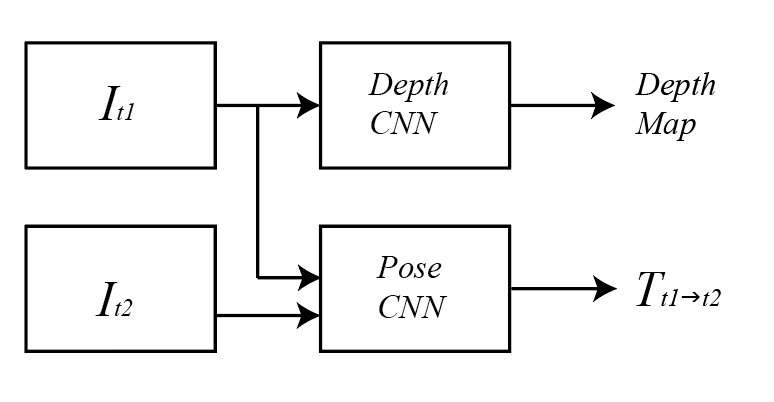
\includegraphics[width=3in]{images/cnns.png}
    \caption[A pair of neural networks for learning depth and pose]{Machine learning approaches have demonstrated strong results in simultaneously estimating depth maps and relative poses between images. Typically, a pair of CNNs is used, one for each task. The depth CNN is provided with the first view at $t=1$ and the pose CNN is provided both views.}
    \label{2cnns}
\end{figure}


While the training pipeline is unsupervised in the sense that labelled data is not required, some form of supervision signal is nevertheless required to optimise the parameters of the pair of networks. These papers take advantage of the fact that if the physical structure of a scene is known, then a novel rendering of that scene from a different viewpoint is achievable. Thus, \cite{garg2016unsupervised} suggested using photometric reconstruction as a supervision signal - from $I_{t2}$, reconstruct $I_{t1}$. The difference between the reconstruction and the real image can form a supervisory signal for the pair of networks. This work similarly uses photometric reconstruction as the principal supervisory signal in training a pair of networks to perform visual odometry and depth estimation. The photometric reconstruction loss is


\begin{equation}
    L_{photometric} = \sum_n^W \sum_m^H |I_{t1}(m,n) - \hat{I_{t1}}(m,n)|.
    \label{photometricloss}
\end{equation}


Humans can easily imagine what a scene will look like if we move our heads slightly, but only if we know the overall shape of the object we are looking at. Similarly, given two images separated by a small interval of time $I_{t1}$ and $I_{t2}$, one could synthesise what $I_{t1}$ would look like by sampling the pixels from $I_{t2}$, if the relative pose $T_{t1\rightarrow t2}$ between the two cameras and a pixel-wise depth of the scene $D_{t1}(p)$ is known. In practice, this can be done by obtaining the coordinates of the pixels in the first image $p_{t1}$ projected on to $I_{t2}$'s camera sensor. Assuming a pinhole model, the complete expression for $p_{t1}$'s projected location on the second camera, $\hat{p_{t2}}$ is 

\begin{equation}
\hat{p_{t2}} = KT_{t1\rightarrow t2} D(p_{t1}) K^{-1} p_{t1}.
\end{equation}
Here K represents the intrinsics matrix. In right-to-left order, this transform first maps each pixel to a ray direction using the inverse camera intrinsics $K^{-1}$. Each ray is then assigned a z-coordinate using the per-pixel depth map $D(p_{t1})$, producing a 3D point cloud. The transform $T_{t1 \rightarrow t2}$ transforms each point to the coordinate frame of the second camera, then the matrix $K$ projects each of those points onto the camera sensor of the second camera. The obtained coordinate $\hat{p_{t2}}$ is continuous, while pixel coordinates are discrete. A pixel value thus needs to be interpolated, keeping in mind that each step of a neural network pipeline must be differentiable to support the backpropagation of gradients. 

It was suggested by Zhou et al. \cite{zhou2017unsupervised} that adopting bilinear sampling could be used as a fully differentiable sampling mechanism. The use of bilinear interpolation as a differentiable sampling pipeline was first proposed Jaderberg et al. \cite{jaderberg2015spatialtransformer}, and adapted by Zhou et al. \cite{zhou2017unsupervised} to perform the differentiable image warp. A bilinear sampling kernel is described by 

\begin{equation}
    V = \sum_n^W \sum_m^H U_{nm} max (0, 1-|x - n|) max(0, 1-|y - m|).
\end{equation}
$V$ is the output of the sampling kernel, $U$ is the source image being sampled, $n$ and $m$ index over the columns and rows of the kernel respectively, $H$ and $W$ are the height and width of the sampling kernel, and $x$ and $y$ are the local coordinates of the sampling location. The $2 \times 2$ sampling kernel used to perform the photometric reconstruction is, in essence a weighted sum of the 4 nearest neighbour pixels, based on its proximity to those pixels. The equation is differentiable with respect to both x and y:


\begin{equation}
    \frac{\partial{V}}{\partial{x}} = \sum_n^W \sum_m^H U_{nm} max(0, 1-|y - m|).
\end{equation}
\begin{equation}
    \frac{\partial{V}}{\partial{y}} = \sum_n^W \sum_m^H U_{nm} max(0, 1-|x - n|).
\end{equation}
Using this bilinear sampling kernel, we can thus sample pixels from $I_{t2}$ to reconstruct $I_{t1}$ in a fully differentiable manner, allowing the backpropagation of gradients through the networks. The pipeline with photometric reconstruction as the supervision signal can be illustrated as shown in Figure \ref{supervisedMLCNNS}. Bilinear interpolation is similarly employed in this work to compute the photometric reconstruction loss of the estimated depth and pose. However, because this work operates on light fields, the output of photometric reconstruction won't be a single image, but a whole array of images.


\begin{figure}
    \centering 
    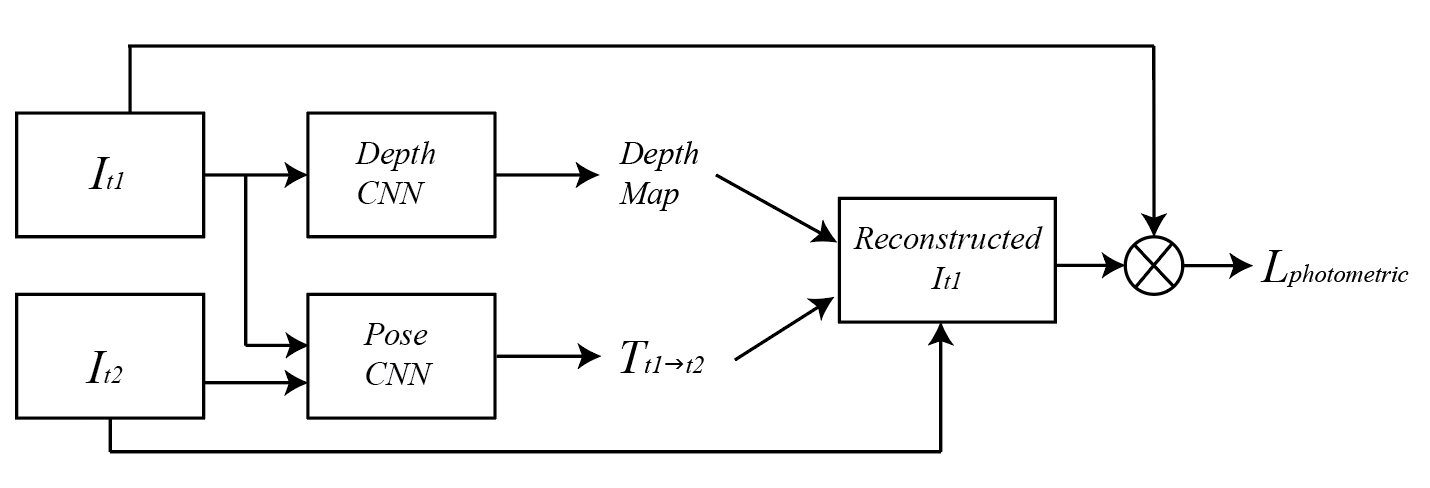
\includegraphics[width=5in]{images/mlpipeline.png}
    \caption[A network architecture for computing photometric loss from depth and pose]{To provide a supervisory signal to the depth and pose CNNs, Garg et al. \cite{garg2016unsupervised} suggested using photometric reconstruction. The loss function is formulated by taking the difference between the reconstructed image $\hat{I_{t1}}$ and the actual image $I_{t1}$, shown in equation \ref{photometricloss}.}
    \label{supervisedMLCNNS}
\end{figure}


In addition to the photometric reconstruction loss providing the main supervision signal to the network, Zhou et al. \cite{zhou2017unsupervised} employs a smoothness loss to ensure that the produced depth map is globally smooth. The smoothness penalises the second order gradient of the image - i.e. the depth network is encouraged to produce a depth map characterised mostly by low-frequency components, and penalised for high-frequency components. Recognising that depth discontinuities frequently occur in parts of the image where a strong edge appears, Godard et al. \cite{godard2016consistency} on the other hand suggested the use of an edge-aware smoothness loss that also penalises large gradients in the depth map $\partial{d}$, but lowers the weight of the loss in regions where the image gradient $\partial{I}$ is large. 

\begin{equation}
    L_{smooth} =  \sum_n^W \sum_m^H |\partial_x d_{nm} e^{-|\delta_x I_{nm}|}| + \partial_y d_{nm} e^{-|\delta_y I_{nm}|}|
\end{equation}

There have been several iterations \cite{bian2019consistency, godard2016consistency, godard2018selfsupervised, zhan2018deepfeature} of this pipeline, most of which have focussed on introducing novel loss functions to improve the quality of the depth and pose estimates. To the best of our knowledge however, this pipeline has only been applied to monocular and stereo camera imagery. While monocular and stereo cameras are ubiquitous in modern digital devices, this thesis drives the investigation further, studying the potential for the use of similar pipelines to achieve improved results using a broader, more generalised family of imaging devices. 

Breaking free of the pinhole principle from which human eyes have developed and which commercial cameras have adopted, has wide implications in the field of machine vision. Reinforcing this idea is the rise in popularity of imaging techniques such as multi-spectral imaging, plenoptic cameras and polydioptric cameras, however interpreting ray directions and geometry for new cameras may not always be apparent, giving rise to the data-driven approach. Working on the principle that machine vision does not necessitate mimicking the human eye to capture imagery, this thesis investigates the capabilities of machine learning for querying depth and pose using one such novel imaging device - a camera array.



\section{Convolutional Neural Networks and Light Fields}


Crafting a data-driven pipeline for visual odometry and depth requires a neural architecture that is capable of ingesting light field data. Importantly, the shape of the data must be considered. Our parameterisation of the light field has four dimensions, denoted by \textit{S, U, T, V}. Convolutional neural networks normally operate on 2D image data, meaning the search for a suitable neural architecture is an important step in testing this work's hypotheses (convolutions in 3 and 4 dimensions are also possible, however they incur significant computational overhead, and for reasons that will become apparent in the next chapter, are difficult to apply to our specific image data).


Wang et al. \cite{wang2016lfcnn} exploit the rich textural information contained in the light field, applying a convolutional network to the task of material classification using light field imagery. In addition to reporting significantly better accuracy compared to 2D imagery (with gains of over 7\%), \cite{wang2016lfcnn} suggests 5 novel methods for interpreting light field data for convolutional networks. One of Wang's most promising architectures, which is referred to in their paper as using interleaved `spatial' and `angular' kernels, exploits the fact that presenting light field data in a different order exposes new kinds of information. 

As discussed in \cite{dansereau2014phd}, a 4D light field image may be tiled as a 2D grid of 2D projective images (called \textit{(u,v)} slices). Alternatively, the light field may be tiled as a 2D grid of 2D \textit{orthographic} images, as seen in Figure 3.4. By presenting the image data to their network in the two different forms as shown in Figure 3.3, Wang et al. approximates convolution in 4 dimensions, allowing their network to learn a 4D signal processing function without the computational overhead of convolving in 4 dimensions.

\begin{figure}
    \centering 
    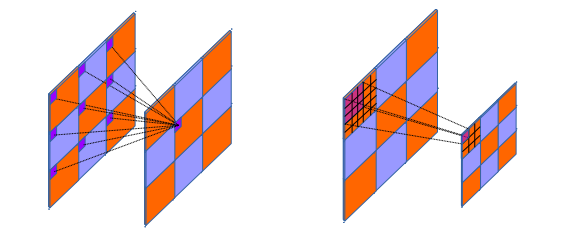
\includegraphics[width=3.5in]{images/spatial-angular.png}
    \caption[Spatial and angular convolutional filters for convolving over light fields]{Adapted from \cite{wang2016lfcnn}, this figure shows convolutions in the angular and spatial dimensions of the light field. Angular Filters (left): by fixing the coordinate \textit{(u, v)} and varying \textit{(s, t)}, the 2D grid of images can be presented to a neural network in the form of orthographic images. Spatial Filters (right): instead of fixing \textit{(u, v)} coordinates, \textit{(s, t)} is fixed while \textit{(u, v)} is varied. This presents information to the neural network as a grid of perspective images.}
    \label{spatial-angular}
\end{figure}


\begin{figure}
    \centering 
    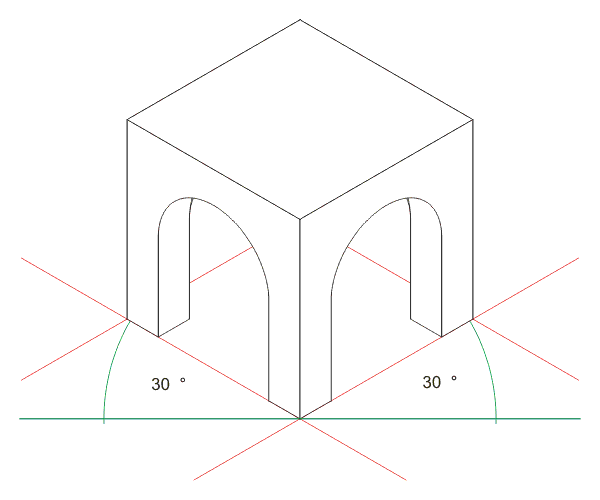
\includegraphics[height=1.7in]{images/orthographic.png}
    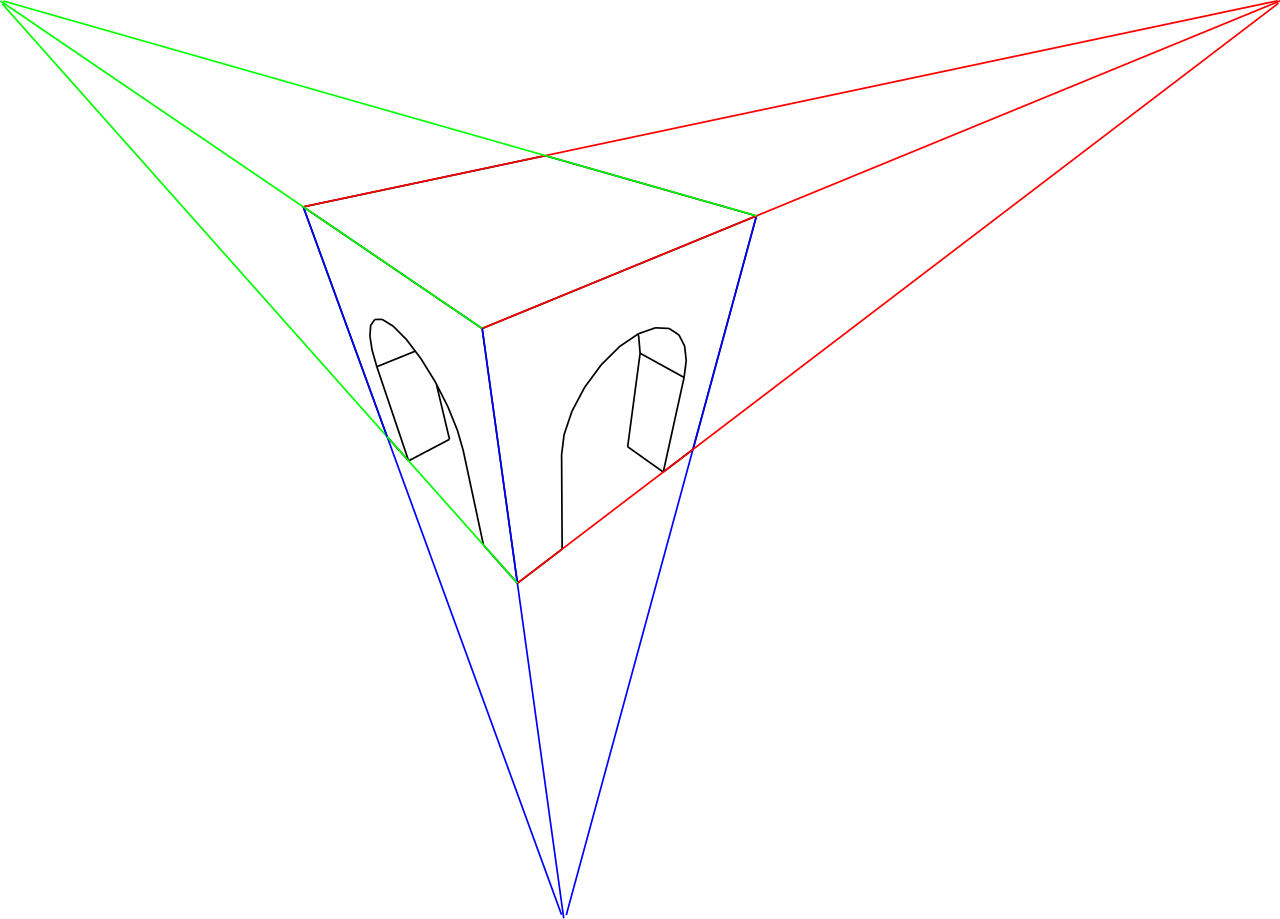
\includegraphics[height=1.7in]{images/perspective.png}
    \caption[Orthographic and pinhole projection images]{Orthographic projection (left) \cite{behrendt2006isometric}: the lines of sight to all points in the scene are parallel to one other, and perpendicular to the projective plane. Perspective projection (right) \cite{gothe2009perspective}: lines of sight converge to a point giving the effect that distant objects appear smaller than nearby objects.}
\end{figure}

There are some hurdles in this approach that make it challenging to apply in our depth and visual odometry pipeline. Most importantly, arranging the light field as orthographic images is impossible with our specific camera without introducing significant redundant data. The challenge arises from the shape of the camera array. As shown in Figure 2.4, our camera has sub-apertures arranged in a cross-hair formation, meaning the complete 2D grid of 2D images is unavailable to us. In the following chapter, we will describe a novel technique that, similar to Wang et al. approximates convolution in 4 dimensions by presenting light field data in a different order to the ordinary \textit{(u, v)} slices that we are familiar with.

Wang et al. suggests another suitable architecture for application in this work, which involves stacking the images along their colour-channels, feeding the data to a convolutional network as a cuboidal volume. This approach is a simple and intuitive way of arranging the light field data, however neural networks may not be able to take full advantage of the 4D signals in light field data this way. Nevertheless, it is a useful way of representing the light field, especially as a format which is easily prepared for ingestion by CNNs, and is thus also explored as an input format in this work's experiments.


\section{Learning Depth From Light Fields}

In Section 3.2.1 we briefly touched on many of the experiments that have been conducted using the KITTI dataset, including two approaches for the supervised learning of depth from monocular imagery. We extend on that discussion in this section, describing in more detail some of the approaches for learning depth from light fields, rather than monocular imagery. This is a relevant and important part of the literature to understand, as depth estimation forms an integral part of our visual odometry pipeline. 

Almost all learning based approaches employ convolutional neural networks - they have been shown time and again to perform well on image data. Within the CNN family of learning-based depth estimation, we distinguish between work that uses 2D convolutional neural networks, and those using convolutions in 3 or more dimensions. 

Within the 2D family of algorithms, Heber \textit{et al.} \cite{heber2017shape} was the first to suggest a deep learning based method for depth estimation from light fields. Their approach used a CNN to learn an end-to-end mapping between the 4D light field and 2D hyperplane orientations - which translate directly to depth. 

Epipolar plane images (EPIs) are employed frequently in 2D methods - EPIs directly encode depth as simple 2D features, making them an attractive input format for depth estimation. For example, Sun \textit{et al.} \cite{sun2016lfdepthcnn} suggest an enhanced EPI feature that encodes scene depth at each point in the light field, which they use to estimate depth using a supervised CNN. Leistner \textit{et al.} \cite{leistner2019lfdepthcnn} takes this one step further, generalising the use of EPIs for learning depth from wide-baseline light fields. Using a strategy which they describe as \textit{EPI-shift}, their technique reduces the size of the convolutional receptive-field needed to detect especially shallow slopes, which are characteristic of wide-baseline light field cameras. Shin \textit{et al.} \cite{shin2018epinet} extend the use of EPIs for depth, by also incorporating the diagonally constructed EPIs for a total of 4 individual EPI feature maps. Each of these is encoded by a separate feature extractor, where features are subsequently concatenated and fed to a secondary CNN which outputs disparity predictions. 

Light fields are typically represented as a 2D array of 2D images, begging the question, why are higher-dimensional convolutions not frequently used? This approach has indeed been suggested, by Faluvégi \textit{et al.} \cite{faluvegi2019threedcnn} who use a fully-convolutional 3D CNN to predict disparity from light field images, demonstrating results that are competitive with the state-of-the-art. On the other hand, 3D convolutions are computationally expensive, and many of the benefits of 2D CNNs are lost - such as the ability to use pre-trained networks or the ability to employ existing 2D architectures. 

\section{Summary}
In this chapter, we've introduced the idea of odometry and depth perception as two challenging tasks which might be addressed with visual sensors. We followed this discussion with a survey of current state-of-the-art methods - which we have broken into two categories - the \textit{geometric} approach which emphasises mathematically modelling the geometry of a moving camera, and the \textit{data-driven} approach which instead fits a non-linear approximation model to large datasets. This work addresses a challenging problem, that is not addressed in any of the methods we have surveyed - the ability to learn depth and odometry from an uncalibrated camera array. We approach this problem in this work, by suggesting a flexible algorithm that, in principle, operates on arbitrarily large arrays of cameras. Furthermore, our algorithm combines successes from both geometric and data-driven families of algorithms, occupying a niche that draws on the success of plenoptic imaging, and the self-supervising features of machine learning approaches. Previous work had not suggested any methods for estimating depth and pose using uncalibrated camera arrays - in Chapter 4, we will outline in detail the operation of our suggested algorithm to overcome this shortcoming using unsupervised learning. This algorithm will bring robotics one step closer towards autonomy in environments where adverse effects such as shock and vibration are punishing for camera calibrations. In Chapter 5 we apply both qualitative and quantitative analysis to the results of our proposed pipeline. 